\documentclass{article}
% Display lists (DESIGN 4.5, `PARTEX_DISPLAY=1`): xtask's `display` job
% checks each page's list against the PDF's content stream as pdftext
% reads it. Text in fonts and sizes (two sizes of one PDF font), math,
% rules (thick, thin, a table's), colors, a turned and a scaled box,
% TikZ paths, an opacity and a turned node, a form drawn twice, an
% included PDF page, a PNG image, literals in each mode, a turned page.
\usepackage{xcolor}
\usepackage{graphicx}
\usepackage{tikz}
\begin{document}
\section{Fonts and rules}
Plain text, \textbf{bold}, \textit{italic}, {\small small} and {\Large
large}, $x^2 + \sqrt{y}$ and $\frac{a}{b}$.
\rule{2cm}{0.2pt} \rule{1cm}{3pt} \rule{0.3pt}{1cm}

\begin{tabular}{|l|r|}\hline A & 1 \\ \hline B & 2 \\ \hline\end{tabular}

\textcolor{red}{Red text} and \colorbox{yellow}{a box}.

\rotatebox{30}{Turned text \rule{1cm}{2pt}} \scalebox{1.5}{Scaled}

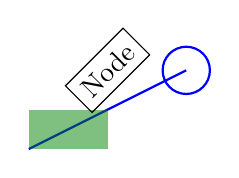
\begin{tikzpicture}
  \draw[blue, thick] (0,0) -- (2,1) circle (0.3);
  \fill[green!50!black, opacity=0.5] (0,0) rectangle (1,0.5);
  \node[rotate=45, draw] at (1,1) {Node};
\end{tikzpicture}

\setbox0\hbox{\textcolor{blue}{Form text}}\immediate\pdfxform0
\pdfrefxform\pdflastxform{} and \pdfrefxform\pdflastxform.
\pdfliteral page{q 0.5 g Q}\pdfliteral direct{}Text after literals.

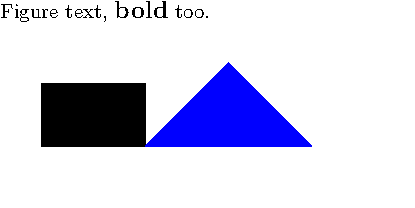
\includegraphics[width=3cm]{images-fig}

\includegraphics[width=1cm]{png-rgb8}

\newpage
\pdfpageattr{/Rotate 90}
A turned page.
\end{document}
